%
%
%
\chapter{The Static Conductivity in the Spin Fermion Model including Umklapp Scattering}
\label{ch:calculation}
%
%
%
The static electrical conductivity $\sigma_{\mt{dc}}$ is computed in this chapter, using the memory-matrix-formalsim.
The underlying model is the spin-fermion-model (see chapter \ref{ch:spin fermion model}), including umklapp scattering as a translation symmetry breaking pertubation.
In this chapter, our attention is focused on the physical analysis of the obtained expression for the conductivity.
An explicite computation is demonstrated in appendix \ref{app:calculation}
%
%
%\section{Static Conductivity's Derivation}
%\label{sec:deviation conductivity}
%
%
Two physical objects, fermions near the Fermi surface and spin fluctuations, are considered in the spin-fermion-model, introduced in the previous chapter.
Spin fluctuations are generated at the vicinity of an antiferromagnetic quantum critical point due to particle-holes-excitations.
Fermions, located at the point $\vb{k}$ and $\vb{k}+\vb{Q}$ on the Fermi suface, are connected to each other because of these fluctuations.
In the previous chapter, it is shown that the model Hamiltonian of the spin-fermion-model is conserved the momentum.
The static electrical conductivity is thus infinite as it is poven in chapter \ref{ch:infinite conductivity}.
Considering umklapp scattering, the translation symmetry is broken and the momentum is unconserved.
As a conseuqence the static conductivity becomes finite, which is computed in the following.

In chapter \ref{ch:memory matrix formalism} over the memory-matrix-formalism, the following formula is derivated for the static electrical conductivity, considering the spin-fermion-model and umklapp scattering.
%
\begin{align}
	\sigma_{\mt{dc}} = \lim\limits_{z \to 0} \frac{z \cdot |\chi_{\mt{JP}}(\omega = 0)|^{2}}{\mathcal{G}_{\dot{\mt{P}}\dot{\mt{P}}}(\vb{k}, z)}
\end{align}
%
Here, $z$ is a complex frequency and $\chi_{\mt{JP}}(\omega = 0)$ is the static susceptibility between current and momentum.
In the denominator the Green function is given by
%
\begin{align}
	\mathcal{G}_{\dot{\mt{P}}\dot{\mt{P}}}(\vb{k}, z) = \int\limits_{0}^{\infty} \dd{t} e^{izt} \expval{\comm{\dot{\mt{P}}(t)}{\dot{\mt{P}}(0)}_{-}}_{0},
\end{align}
%
where the usual quantum mechanical commutator is used, indicated with the minus sign at the squared brackets.
The expectation value is generated with respect to the unpertubative Hamiltonian H, illustrated with the index 0.
Here, the interaction between fermions and spin fluctuations is included.
The time derivative of momentum is given by equation \eqref{eq:time derivative momentum finite}.

The Green function $\mathcal{G}_{\dot{\mt{P}}\dot{\mt{P}}}(\vb{k}, z)$ and the static susceptibiliy $\chi_{\mt{JP}}(\omega = 0)$ are investigated, due to their possible temperature dependence.
The latter is expected to be temperature independent.
\todo{Why? -> P and J are explicitely time independent}
This is computed in detail in the appendix \ref{app:calculation}, using the diagrammatic pertubation technique.
The considered diagrams are the electron-pair bubble for each species of fermions, depicted in figure \ref{fig:bubble electrons}.
Therefore, the obtained expression of the susceptibility is given by
%
\begin{align}
	\chi_{\mt{PJ}}(\omega = 0) = \frac{\sqrt{m_{1} m_{2}}}{\pi} T \cdot \ln(e^{\flatfrac{\mu}{T}} + 1),
\end{align}
%
where the chemical potential is denoted as $\mu$.
The logarithm is approximated in the limit of small temperatures ($\mu \gg T$) to $\ln(e^{\flatfrac{\mu}{T}} + 1) \rightarrow \flatfrac{\mu}{T}$.
Inserting this expression, the temperature is canceled and the static susceptibility is given by constant parameters, $\chi_{\mt{PJ}}(\omega = 0) = \flatfrac{\mu\sqrt{m_{1} m_{2}}}{\pi}$.
The chemical potential is assumed as temperature independent in the observed regime.

%
\begin{figure}
	\centering
	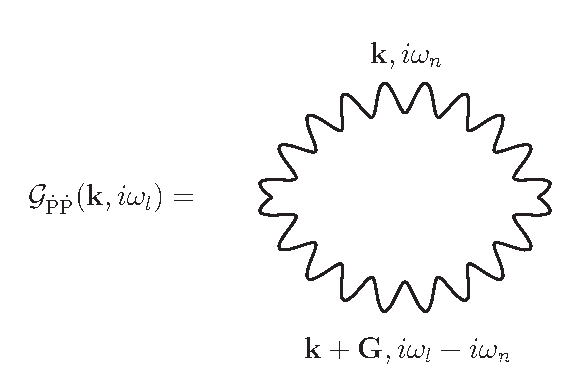
\includegraphics[width=0.4\textwidth]{spin_wave_bubble.eps}
	\caption{caption}
	\label{fig:spin wave bubble}
\end{figure}
%
The only temperature dependence of the static electrical conductivity is hence emerged by the Green function $\mathcal{G}_{\dot{\mt{P}}\dot{\mt{P}}}(\vb{k}, z)$.
Only the free bubble diagram is considered computing the Green function with diagrammatic pertubation theory, which is depicted in figur \ref{fig:spin wave bubble}.
Higher order terms in the diagrammatic treatment are corrections of the bubble diagram and since spin fluctuations are the observing objects only bubble diagrams occur.
Therefore the conductivity or resistance is only determined by spin fluctuations.
Resistance is a consequence of fermionic coupling to other degrees of freedom, obtained as finite fermionic lifetime.
The resistance is thus proportional to the imaginary part of the retarded Green function $\mathcal{G}_{\dot{\mt{P}}\dot{\mt{P}}}^{\mt{ret}}(\vb{k}, z)$.
Appendix \ref{app:calculation} is shown the detailed computation of the expression of the retarded Green function.
%
\begin{align}
	\Im{\mathcal{G}_{\dot{\mt{P}}\dot{\mt{P}}}^{\mt{ret}}(\vb{k}, z)} &= 
		-\frac{4 \gamma^{2} \beta \omega}{\pi}
		\sum\limits_{\vb{Q}_{1}, \vb{Q}_{2}}
		\sum\limits_{\vb{G}}
		\vert \mt{J}_{\vb{G}} \vert^{2}
		\int\limits_{0}^{\infty} \dd{\epsilon}
		\frac{\epsilon^{2} e^{\beta \epsilon}}{(e^{\beta \epsilon} - 1)^{2}}
		\notag \\
		&\times
		\int_{\vb{k}} G_{j}^{2} \cdot
		\frac{1}{(\vb{k}+\vb{G}-\vb{Q}_{1})^{4} + \gamma^{2} \epsilon^{2}} \cdot
		\frac{1}{(\vb{k} + \vb{Q}_{2})^{4} + \gamma^{2} \epsilon^{2}}
\end{align}
%
Here the term under the momentum integral is given by the imaginary part of the damped spin density propagator, denoted in \eqref{eq:damped spin propagator real axis}.
The integral itself is extended over the first Brillouin zone.
The periodicity of the spin susceptibility and pertubation is considered by the sums over $\vb{Q}_{i}$ ($i=1,2$) and $\vb{G}$, respectivily.
In both cases these are reciprocal lattice vectors.
Spatial direction of the momentum is represented by the index $j$ and $\beta^{-1} = T$.

The obtained integrals is now investigated with respect to different cases since their are not exactly solvable.
A detailed discussion of the single cases and an approximated computation of the integral is demonstrated in the following.

%
%
%\section{Analysis of the static conductivity}
%\label{sec:analysis conductivity}
%
%
Convergence of the intergal is surely given, if one of the momentum terms, $\vb{k}+\vb{G}-\vb{Q}_{1}$ or $\vb{k} + \vb{Q}_{2}$, is large according to amount.
Since both terms are of the power of four, the integral is a fast decreasing function in the large momentum limit.
Nevertheless, divergences of the integral are reached, if these terms are zero and this happens in many cases.
One of the most divergent cases is assumed in the following approach.
The vector $\vb{k}$ is limited on the first Brillouin zone and the reciprocal lattice vectors are set to $\vb{G} = \vb{Q}_{1}$ and $\vb{Q}_{2} = 0$.
The choice of the reciprocal lattice vectors is arbitrary and it is therefore possible that the $j$-component of $\vb{G}$ is large.
This divergence is killed by the coupling parameter $\mt{J}_{\vb{G}}$ assumed as fast decreasing for large $|\vb{G}|$.

The remaining momentum integral is now exactly integrable.
First of all, the momentum and frequency variables are transformed into dimensionles variables, using the transformation rules $\vb{k} = \vb{y} \cdot \sqrt{\gamma T}$ and $\epsilon = x \cdot T$, respectivily.
The new variable $\vb{y}$ is further transformed into plane polar coordinates.
The upper limit of the radius $|\vb{y}|$ is set to infinity, since the integrand is decreasing fast to zero for $|\vb{y}| \to \infty$.
As a consequence the angular integral is easily evaluated, yielding the factor $2\pi$.
The remaining integral is given by the following expression.
%
\begin{align}
	\Im{\mathcal{G}_{\dot{\mt{P}}\dot{\mt{P}}}^{\mt{ret}}(\vb{k}, z)} = 
		 -\frac{2 \cdot G_{j}^{2} \cdot \vert \mt{J}_{\vb{K}} \vert^{2}}{\gamma \cdot \pi^{2}} \cdot \frac{\omega}{T}
		\int\limits_{0}^{\infty} \dd{x}
		\frac{x^{2} e^{x}}{(e^{x} - 1)^{2}}
		\int\limits_{0}^{\infty} \dd{y}
		\frac{y}{\big(y^{4} + x^{2}\big)^{2}}
\end{align}
%
The $y$-integral is substituted one last time, using the transformation rule $y^{2} = z \cdot x$.
The obtained integral is evaluated to $\flatfrac{\pi}{4}$, using the integral formula \eqref{eq:integral1}.
Both limits, $x \to 0$ and $x \to \infty$, of the intergal over $x$ are investigated.
In the case of large $x$, the integral is decreasing fast to zero due to the ratio of the exponential functions.
The upper limit is thus set to one and the integrand is expanded for small values of $x$.
In first order the integrand is approximated to $\flatfrac{1}{x^{3}}$.
This is a highly divergent function in the limit $x \to 0$.











































